\documentclass[a0,final]{a0poster}
%%%Load packages
\usepackage{multicol} 			%3-column layout
\usepackage[left=2cm,right=2cm,bottom=0cm,top=0cm]{geometry}			%Reset margins
\usepackage{mathpazo}			%Load palatino font & pazo math
\usepackage{color}

\usepackage{amsmath, amsthm, amssymb}

\usepackage{tikz}
\usepackage{tikz-3dplot}
\usetikzlibrary{arrows.meta, cd, fadings, patterns}

\usepackage{pgfplots}
\usepackage[inline]{asymptote}

\usepackage{graphicx}
\usepackage{adjustbox}
\usepackage{dsfont}
\usepackage{booktabs}


\tikzfading[name=fade out, inner color=transparent!0, outer color=transparent!100]



%Needed for colour boxes & coloured text

%%%Define colours and lengths
\definecolor{headingcol}{rgb}{1,1,1}			%Colour of main title
\definecolor{boxcol}{rgb}{0.7,0.2,0.2}		%Edge-colour of box and top banner
\fboxsep=1cm							%Padding between box and text
\setlength{\columnsep}{2cm}				%Set spacing between columns

%%%Format title
\makeatletter							%Needed to include code in main file
\renewcommand\@maketitle{%
\null									%Sets position marker
{
\color{headingcol}\sffamily\VERYHuge		%Set title font and colour
\@title \par}%
\vskip 0.6em%
{
\color{white}\sffamily\large				%Set author font and colour
\lineskip .5em%
\begin{tabular}[t]{l}%
\@author
\end{tabular}\par}%
\vskip 1cm
\par
}
\makeatother

\title{Spectral Sequences and Higher Homotopy Groups of Spheres\hspace*{10cm}

\includegraphics[]{aep-logo-2}}

\author{D. Zack Garza\\
Advised by Justin Roberts \\
University of California, San Diego }

\begin{document}

\hspace{-3cm}								%Align with edge of page, not margin
\colorbox{boxcol}{							%Coloured banner across top
\begin{minipage}{1189mm}					%Minipage for title contents
\maketitle
\end{minipage}}
\vspace{1cm}

\begin{multicols}{3}							%Use 3-column layout
\raggedcolumns							%Don't stretch contents vertically

%%%Column1
\section*{Background}
This project is centered around the use of spectral sequences to compute topological invariants of spaces. These invariants can be used to categorize, study, and distinguish familiar spaces that arise in various branches of Mathematics, and often lead to the construction or discovery of entirely new types of spaces.

Generally speaking, Topology is the study of spaces that admit a notion of closeness, measured by a collection of ``open sets''. Spaces fitting such a description are said to be objects in the category of \textbf{Topological Spaces} (also denoted \textbf{Top}). In this category, spaces are only distinguished up to \textbf{homeomorphism}, a continuous bijective map with continuous inverse. That is, given two spaces and a map $f: X \to Y$, if $f$ is continuous and admits an continuous inverse $f^{-1} X \to Y$, then $X$ and $Y$ are considered equivalent objects in \textbf{Top} and we write $X \cong Y$. Such maps $f$ can also be thought of as continuous deformations from $X$ to $Y$.

Such deformations preserve purely topological properties, such as the number of connected components and the number of holes. Such properties are referred to as \textit{topological invariants}. It is for this reason that Topology is sometimes referred to as ``rubber sheet geometry'', in which the surfaces act like rubber or clay that can be reshaped but can not be torn without potentially affecting its topological properties. An oft-cited example is that, thought of as surfaces embedded in $\mathbb{R}^3$, a coffee cup is homeomorphic to a one-holed torus, and thus there is a continuous map of the following type:

\begin{center}
% Coffee Cup
\begin{tikzpicture}[scale=\textwidth/30cm,samples=200]

% Handle
\begin{scope}[shift=(10:7/8), rotate=-30, yslant=1/2, xslant=-1/8]
  \shade [top color=gray!80, bottom color=gray!30]
    (0,0) arc (130:-100:3/8 and 1/2) -- ++(0,1/4) arc (-100:130:1/8 and 1/4) -- cycle;
  \shade [top color=gray!10, bottom color=gray!60]
    (0,0) arc (130:-100:3/8 and 1/2) -- ++(0,1/32) arc (-100:130:1/4 and 1/3) -- cycle;
\end{scope}

% Cup
\fill [black!75, path fading=fade out]
    (0,-1) ellipse [x radius=3/4, y radius=1/2];
\shade [left color=gray!60, right color=gray!30]
  (-1,0) arc (180:360:1 and 5/4);
\shade [bottom color=gray, top color=gray!30, opacity=1/2]
  (-1,0) arc (180:360:1 and 5/4);
\shade [left color=gray!20, right color=gray!40]
  (0,0) ellipse [x radius=1, y radius=1/2];
\shade [left color=gray!40, right color=gray!20]
  (0,0) ellipse [x radius=1-1/16, y radius=1/2-1/16];
\shade [bottom color=gray, top color=gray!10, opacity=1/2]
  (0,0) ellipse [x radius=1-1/16, y radius=1/2-1/16];
\draw  (0,-1.7) node {$X = $ A Coffee Cup};
\draw[-{Latex[length=3mm,width=3mm]}] (1.5, -.5) .. controls (2, -1) and (2.5, .5)  ..(4.2, -.5);
\draw  (3.0,0) node {$f: X \to Y$};

\end{tikzpicture}
% Torus in R3
\begin{asy}
  size(400);
  import graph3;

  currentprojection=perspective(5,4,4);
  real R=3;
  real a=1;

  triple fs(pair t) {
    return ((R+a*Cos(t.y))*Cos(t.x),(R+a*Cos(t.y))*Sin(t.x),a*Sin(t.y));
  };

  surface s=surface(fs,(0,180),(360,360),8,8,Spline);
  draw(s,surfacepen=material(blue+opacity(0.6), emissivepen=0.2*white),render(compression=Low,merge=true));

  xaxis3(Label("$x$",1),xmin=0,xmax=7,Arrow3);
  yaxis3(Label("$y$",1),ymin=0,ymax=7,Arrow3);
  zaxis3(Label("$z$",1),zmin=0,zmax=4,Arrow3);
  label("$Y = $ A Torus", (0,-40), p = fontsize(30pt));
\end{asy}
\end{center}

The simplest such examples arise from looking at subsets of real $n$-dimensional space, in particular, the solid ball $B^n$ and its spherical shell $S^n$. For low dimensions, these are readily visualized:

\begin{center}
% Spheres
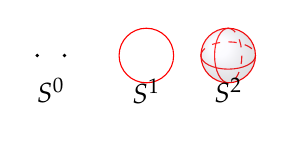
\begin{tikzpicture}[scale=\textwidth/35cm,samples=200]
	\draw (-7,0)[fill=red] circle (.4mm);
	\draw (-6,0)[fill=red] circle (.4mm);
	\draw  (-6.5,-1.3) node {$S^0$};

    \draw[red] (-3,0) circle (1cm);
	\draw  (-3,-1.3) node {$S^1$};

	\draw[red] (-1,0) arc (180:360:1cm and 0.5cm);
    \draw[dashed, red] (-1,0) arc (180:0:1cm and 0.5cm);
    \draw[red] (0,1) arc (90:270:0.5cm and 1cm);
    \draw[dashed, red] (0,1) arc (90:-90:0.5cm and 1cm);
    \draw[red] (0,0) circle (1cm);
    \shade[ball color=blue!10!white,opacity=0.20] (0,0) circle (1cm);
    \draw  (0,-1.3) node {$S^2$};
\end{tikzpicture}
% Balls
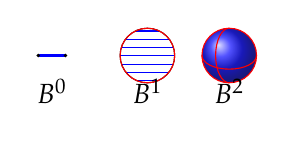
\begin{tikzpicture}[scale=\textwidth/35cm,samples=200]
	\draw[thick, blue] (-7,0) -- (-6,0);
	\draw[fill=red](-6,0) circle (.4mm);
	\draw[fill=red](-7,0) circle (.4mm);
	\draw (-6.5,-1.3) node {$B^0$};

	%\shade[ball color=blue!100!white] (-3,0) circle (1cm);
	\draw[pattern=horizontal lines, pattern color=blue] (-3,0) circle (1cm);
    \draw[red] (-3,0) circle (1cm);
	\draw (-3,-1.3) node {$B^1$};

    \shade[ball color=blue!100!white,opacity=0.90] (0,0) circle (1cm);
    \draw[red] (0,0) circle (1cm);
   	\draw[red] (-1,0) arc (180:360:1cm and 0.5cm);
    \draw[red] (0,1) arc (90:270:0.5cm and 1cm);
    \draw  (0,-1.3) node {$B^2$};
\end{tikzpicture}
\end{center}

There are also a number of other relatively simple spaces that can be assembled by combining these spaces using a variety of product, quotient, and ``twisting'' operations:

\begin{center}
% Cylinder
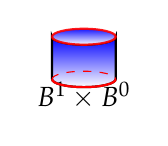
\begin{tikzpicture}[scale=\textwidth/90cm,samples=200]
   \coordinate (ll) at (-3,-2);
   \coordinate (lr) at (3,-2);
   \coordinate (ul) at (-3,2);
   \coordinate (ur) at (3,2);
   \shade [shading angle=90, opacity=0.20] (ll) arc (-180:-60:3cm and .75cm) -- +(0,4) arc (-60:-180:3cm and .75cm) -- cycle;
   \shade [thick, shading angle=270, opacity=0.20, color=red] (lr) arc (0:-60:3cm and .75cm) -- +(0,4) arc (-60:0:3cm and .75cm) -- cycle;
   \draw [thick,top color = blue] (ll) arc (-180:0:3cm and .75cm) -- (ur) arc (0:-180:3cm and .75cm) -- cycle;
   \draw [thick, shade, shading angle=30, opacity=0.90, red, top color = blue] (ul) arc (-180:180:3cm and .75cm);
   \node at (0,-3.5){$B^1 \times B^0$};
    \draw[dashed, red] (-3,-2) arc (180:0:3cm and .75cm);
    \draw[thick, red] (ll) arc (180:360:3cm and .75cm);

\end{tikzpicture}
% Torus
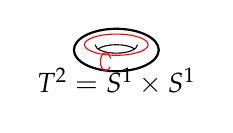
\begin{tikzpicture}[scale=\textwidth/90cm,samples=200]
    \draw[thick] (0,0) arc (0:360: 4cm and 2cm);
    \draw[solid] (-2,.5) arc (0:-180: 2cm and .8cm);
    \draw[solid] (-4,.5) arc (90:150: 2cm and .8cm);
    \draw[solid] (-4,.5) arc (90:30: 2cm and .8cm);
    \draw  (-4,-3) node {$T^2 = S^1 \times S^1$};
    \draw[red] (-4,.5) ellipse (3cm and 1cm);
	\draw[red] (-5,-.25) arc (90:270:.5cm and .85cm);
	\draw[red, dashed] (-5,-.25) arc (90:-90:.5cm and .85cm);
\end{tikzpicture}
% Mobius
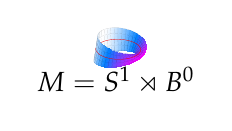
\begin{tikzpicture}[scale=\textwidth/90cm,samples=200]
  \begin{axis}[
    hide axis,
    view = {40}{40}
  ]
  \addplot3 [
    surf,
    colormap/cool,
    shader     = faceted interp,
    point meta = x,
    samples    = 40,
    samples y  = 5,
    z buffer   = sort,
    domain     = 0:360,
    y domain   =-0.5:0.5
  ] (
    {(1+0.5*y*cos(x/2)))*cos(x)},
    {(1+0.5*y*cos(x/2)))*sin(x)},
    {0.5*y*sin(x/2)}
  );

  \addplot3 [
    samples=50,
    domain=-145:180,
    samples y=0,
    thick,
    color = red
  ] (
    {cos(x)},
    {sin(x)},
    {0}
  );
  \end{axis}
  \draw (3,0) node {$M = S^1 \rtimes B^0$};
\end{tikzpicture}
\end{center}


\textbf{Top} also includes a broad array of objects, such as function spaces, collections of matrices, and even large data sets can be given a topological structure. Several natural questions thus arise: \textbf{Can we classify homeomorphism types? And how can we tell when two given spaces are homeomorphic?}

\columnbreak


The size and complexity of \textbf{Top} makes such questions difficult. The \textit{Poincare Conjecture} -- a Millennium Prize Problems which revolved around characterizing when certain 3-dimensional spaces are homeomorphic to the 3-sphere $S^3$ -- remained an open problem for nearly a century until its resolution in 2006. As a result, slightly weaker notion of \textit{homotopy equivalence} was introduced, which began a widely successful program of assigning algebraic invariants to spaces in order to study and distinguish them.

\section*{Homotopy Theory}

The notion of \textit{homotopy} has become a cornerstone of modern Algebraic Topology. As a first approximation, a homotopy between two maps can be thought of as a continuous, time-dependent interpolation between them. In the simplest case, we consider \textbf{paths} within a space $X$ to be equivalent to maps from the unit interval $I$, or equivalently the zero-dimensional ball $B^0$, into $X$, and two maps $f, g: B^0 \to X$ are said to be \textbf{homotopic} whenever there exists a family of maps $F_t: B^0 \to X, t \in [0, 1]$ satisfying $F_0 = f$ and $F_1 = g$. This provides a notion of homotopy between paths in a space.

In this way, the space is ``probed'' by a test space, in this case a ball $B^0$, in order to study it. An extremely useful application of this concept is to measure the number of ``holes'' in a space by taking one's test spaces to be spheres $S^n$ instead of balls. This leads to the notion \textbf{Homotopy Groups}, a collection of groups $\pi_n(X), n = 0, 1, 2, \ldots$ assigned to a space which serve as algebraic invariants: that is, they satisfy the property that $X \cong Y$ implies $\pi_n(X) = \pi_n(Y)$ for all $n$. Conversely, if there is even a single $n$ such that $\pi_n(X) \neq \pi_n(Y)$, one can conclude that $X \not \cong Y$. These groups are defined as
$$\pi_n(X) = [S^n, X]$$
where $[X, Y]$ is obtained by taking the set of all continuous maps $f: X \to Y$ and identifying all maps that are homotopic to one another. We say that two spaces $X$ and $Y$ are \textit{homotopy equivalent} or are equivalent as objects in the category \textbf{hoTop} when there are mutually inverse maps $f: X \to Y$ and $g: Y \to X$ that are each homotopic to the identity maps on the respective spaces.

\begin{center}

%\begin{tikzpicture}[scale=\textwidth/65cm,samples=200, decoration={markings,mark=at position 0.5 with {\arrow{>}}},
   %witharrow/.style={postaction={decorate}}, dot/.style={draw,fill,circle,inner sep=1.5pt,minimum width=0pt}]
\begin{tikzpicture}[scale=\textwidth/65cm, samples=200]
    \draw[thick, blue] (-3,0) -- (-1,0);
	\draw[fill=red](-3,0) circle (.4mm);
	\draw[fill=red](-1,0) circle (.4mm);
	\draw (-2,-.5) node {$B^0$};
    % ellipse
    \node[label={[left] $p$}, red] (a3) at (0,0) {};
    \node[label={[right]$q$}, red] (b3) at (4,0) {};
    \draw[thick,witharrow] (a3) to[out=50,in=150]node[above]{$f$} (b3);
    \foreach \o/\i in {40/160,30/170,20/180,10/190,-10/200}
       \draw[dashed] (a3) to[out=\o,in=\i]  (b3);
    \draw[thick,witharrow] (a3) to[out=-20,in=-145]node[below]{$g$} (b3);
    \draw ($0.5*(a3)+0.5*(b3)$) circle[x radius=2.5,y radius=1.5];
    \node at ($(b3)+(0.5,0.8)$) (X3) {$X$};
    \draw[-{Latex[length=3mm,width=3mm]}] (-2,.2) .. controls (-1.5,3) and (1,1)  .. (1,1);
    \draw[-{Latex[length=3mm,width=3mm]}] (-2,-1) .. controls (-1.5,-3) and (1,-1)  .. (1,-1);
\end{tikzpicture}

\hfill
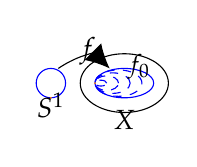
\begin{tikzpicture}[scale=\textwidth/65cm,samples=200]
	\draw[black] (-3,0) ellipse (3cm and 2cm);
    \draw[blue] (-3,0) ellipse (2cm and 1cm);
	\draw[dashed, blue] (-3.4,0) ellipse (1.6cm and .9cm );
	\draw[dashed, blue] (-3.8,0) ellipse (1.2cm and .7cm);
	\draw[dashed, blue] (-4.2,0) ellipse (.8cm and .5cm);
	\draw[dashed, blue] (-4.6,0) ellipse (.4cm and .2cm);
	\fill[orange] (-5,0) circle (.07);
    \draw[-{Latex[length=3mm,width=3mm]}] (-7.5,1) .. controls (-6,2) and (-5,2)  .. (-4,1);
	\draw[blue] (-8,0) circle (1cm);
	\draw  (-8,-1.5) node {$S^1$};
	\draw  (-3,-2.5) node {$X$};
	\draw  (-5.5,2.2) node { $f$};
	\draw  (-2,1.1) node {\small $f_0$};
	\fill[orange] (-8,-1) circle (.07);
\end{tikzpicture}
\end{center}

\subsection*{Maps Between Spheres}
Since spheres are perhaps the simplest spaces to study, we can take both the test space and the target space to both be spheres of varying dimensions. By doing this, $\pi_i(S^n) = [S^i, S^n]$ yields information about homotopy classes of maps between spheres, which might include instances of one sphere winding or wrapping around another. It can be shown that when $i < n$, $\pi_i(S^n) = 0$ -- that is, there is only one class of maps up to homotopy: those that can be contracted to a point. This is most easily visualized by examining $\pi_1(S^2) = [S^1, S^2] = 0$ (the trivial group).

\begin{center}
%Map S^2 to S^2
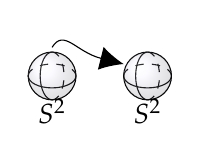
\begin{tikzpicture}[scale=\textwidth/40cm,samples=200]
    \draw (-1,0) arc (180:360:1cm and 0.5cm);
    \draw[dashed] (-1,0) arc (180:0:1cm and 0.5cm);
    \draw (0,1) arc (90:270:0.5cm and 1cm);
    \draw[dashed] (0,1) arc (90:-90:0.5cm and 1cm);
    \draw (0,0) circle (1cm);
    \shade[ball color=blue!10!white,opacity=0.20] (0,0) circle (1cm);

	\draw (-5,0) arc (180:360:1cm and 0.5cm);
    \draw[dashed] (-5,0) arc (180:0:1cm and 0.5cm);
    \draw (-4,1) arc (90:270:0.5cm and 1cm);
    \draw[dashed] (-4,1) arc (90:-90:0.5cm and 1cm);
    \draw (-4,0) circle (1cm);
    \shade[ball color=blue!10!white,opacity=0.20] (-4,0) circle (1cm);

	\draw[-{Latex[length=3mm,width=3mm]}] (-4,1.2) .. controls (-3.5,2) and (-3,1)  .. (-1,.5);
	\draw  (-4,-1.5) node {$S^2$};
	\draw  (0,-1.5) node {$S^2$};
\end{tikzpicture}
\hfill
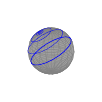
\begin{tikzpicture}[scale=\textwidth/45cm,samples=200]
\begin{axis}[hide axis, axis equal, samples=15]

\addplot3 [surf, gray, faceted color=gray, opacity=0.5, samples=20, z buffer=sort, domain=0:360, y domain=0:1] ({cos(x)*y},{sin(x)*y},
{sqrt(1-(cos(x)*y)^2-(sin(x)*y)^2))});

\addplot3 [surf, gray, faceted color=gray, opacity=0.5, samples=20, z buffer=sort, domain=0:360, y domain=0:1] ({cos(x)*y},{sin(x)*y},
{-sqrt(1-(cos(x)*y)^2-(sin(x)*y)^2))});

\pgfmathsetmacro{\a}{90.0}
\pgfmathsetmacro{\b}{30.0}
\pgfmathsetmacro{\c}{-15.0}

\addplot3 [blue, thick, domain=0:360, samples=20] (
        {(sin(\a)*cos(\b)*cos(\c))*cos(x)+(sin(\a)*sin(\c))*sin(x)-(cos(\a)*sin(\b)*cos(\c))},
        {-(sin(\a)*cos(\b)*sin(\c))*cos(x)+(sin(\a)*cos(\c))*sin(x)+(cos(\a)*sin(\b)*sin(\c))},
        {(sin(\a)*sin(\b))*cos(x)+cos(\a)*cos(\b)}
    );

\pgfmathsetmacro{\a}{60.0}
\addplot3 [blue, domain=0:360, samples=20] (
        {(sin(\a)*cos(\b)*cos(\c))*cos(x)+(sin(\a)*sin(\c))*sin(x)-(cos(\a)*sin(\b)*cos(\c))},
        {-(sin(\a)*cos(\b)*sin(\c))*cos(x)+(sin(\a)*cos(\c))*sin(x)+(cos(\a)*sin(\b)*sin(\c))},
        {(sin(\a)*sin(\b))*cos(x)+cos(\a)*cos(\b)}
    );

\pgfmathsetmacro{\a}{30.0}
\addplot3 [blue, domain=0:360, samples=15] (
        {(sin(\a)*cos(\b)*cos(\c))*cos(x)+(sin(\a)*sin(\c))*sin(x)-(cos(\a)*sin(\b)*cos(\c))},
        {-(sin(\a)*cos(\b)*sin(\c))*cos(x)+(sin(\a)*cos(\c))*sin(x)+(cos(\a)*sin(\b)*sin(\c))},
        {(sin(\a)*sin(\b))*cos(x)+cos(\a)*cos(\b)}
    );

\pgfmathsetmacro{\a}{10.0}
\addplot3 [blue, domain=0:360, samples=10] (
        {(sin(\a)*cos(\b)*cos(\c))*cos(x)+(sin(\a)*sin(\c))*sin(x)-(cos(\a)*sin(\b)*cos(\c))},
        {-(sin(\a)*cos(\b)*sin(\c))*cos(x)+(sin(\a)*cos(\c))*sin(x)+(cos(\a)*sin(\b)*sin(\c))},
        {(sin(\a)*sin(\b))*cos(x)+cos(\a)*cos(\b)}
    );

\pgfmathsetmacro{\a}{5.0}
\addplot3 [blue, domain=0:360, samples=10] (
        {(sin(\a)*cos(\b)*cos(\c))*cos(x)+(sin(\a)*sin(\c))*sin(x)-(cos(\a)*sin(\b)*cos(\c))},
        {-(sin(\a)*cos(\b)*sin(\c))*cos(x)+(sin(\a)*cos(\c))*sin(x)+(cos(\a)*sin(\b)*sin(\c))},
        {(sin(\a)*sin(\b))*cos(x)+cos(\a)*cos(\b)}
    );

\pgfmathsetmacro{\a}{1.0}
\addplot3 [blue, domain=0:360, samples=3] (
        {(sin(\a)*cos(\b)*cos(\c))*cos(x)+(sin(\a)*sin(\c))*sin(x)-(cos(\a)*sin(\b)*cos(\c))},
        {-(sin(\a)*cos(\b)*sin(\c))*cos(x)+(sin(\a)*cos(\c))*sin(x)+(cos(\a)*sin(\b)*sin(\c))},
        {(sin(\a)*sin(\b))*cos(x)+cos(\a)*cos(\b)}
    );
\end{axis}
\end{tikzpicture}
\end{center}
\subsection*{$\pi_{n} S^n = \mathbb{Z}$}

For each $n$, it can be shown that there are in fact infinitely many nontrivial classes of maps from the $n$-sphere to itself, and it can be show that $[S^n, S^n] \cong \mathbb{Z}$. The prototypical example of this is in dimension 1, where the construction of a \textit{covering space} yields a method of computing $[S^1, S^1] = \pi_1(S^1)$. It can be shown that $\mathbb{R} \twoheadrightarrow S^1$ is such a covering, which can be visualized as a helix over the circle, where the degree is measured by the \textit{winding} or equivalently the number of points in the fiber above a base point:

\tdplotsetmaincoords{70}{15}
\tikzset{every circle/.append style={x=1cm, y=1cm}}

\begin{center}
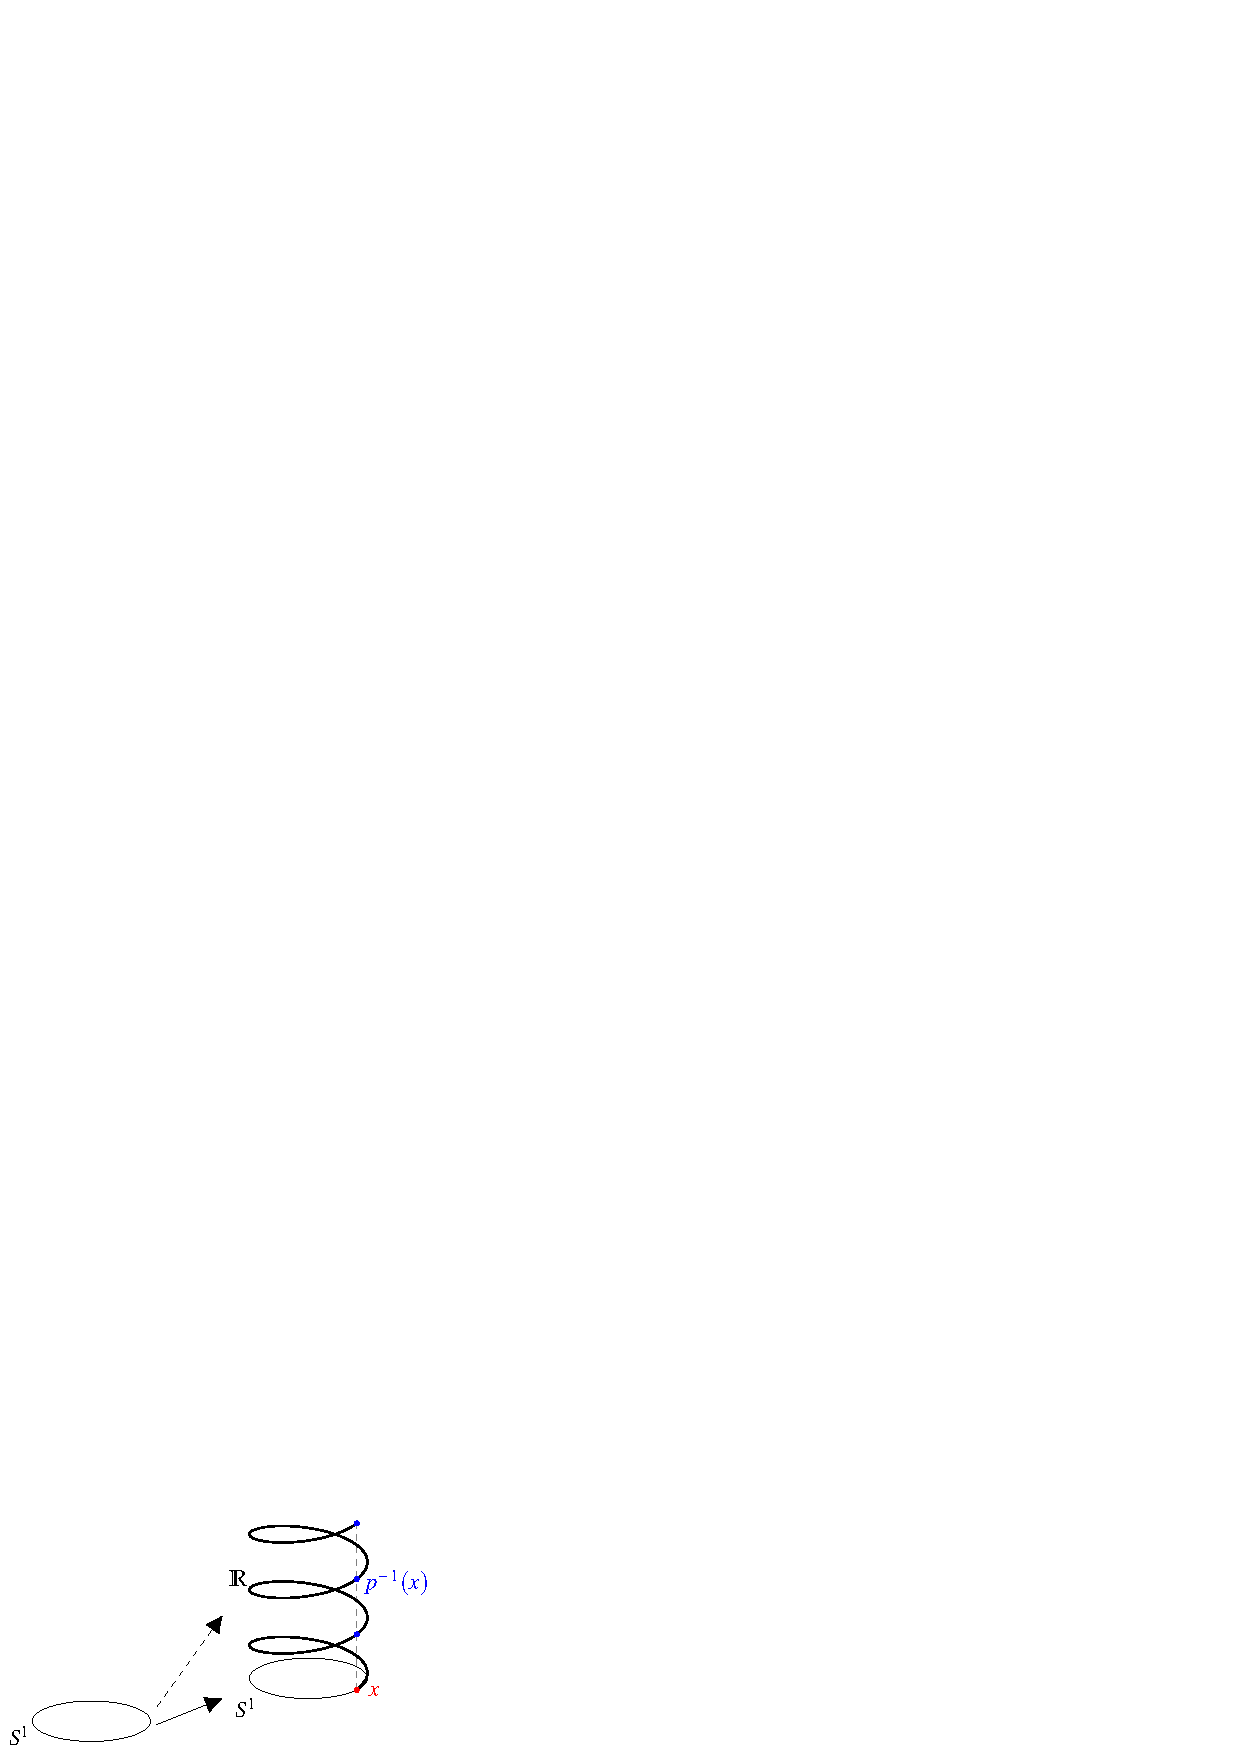
\includegraphics[width=20cm]{helix}
\end{center}


\subsection*{Spectral Sequences}
Spectral sequences are a tool for computing \textit{homology}, another algebraic invariant. When combined with a construction called \textbf{Postnikov Towers}, which generalize the construction of covering spaces, these sequences can also be used in an iterative procedure to compute homotopy groups. These sequences are represented as a differential graded structure $(E_n^{p,q}, \partial_n^{p,q})$ in which each $E_n$ (denoted the \textit{pages} of the sequence) is obtained from the previous page by taking homology. This induces differentials that extend farther on each page, and with further assumptions on the boundedness of this complex, the pages stabilize and the sequence is said to converge.


\adjustbox{scale=.5,center}{%
$E_1$:
\begin{tikzcd}
q ~/~ F & \cdot \arrow[r, "{d_2^{0,2}}"] & \cdot \arrow[r, "{d_2^{1,2}}"] & \cdot \arrow[r, "{d_2^{2,2}}"] & \cdot \arrow[r, "{d_2^{3,2}}"] & \cdot &  \\
1 & \cdot \arrow[r, "{d_2^{0,1}}"] & \cdot \arrow[r, "{d_2^{1,1}}"] & \cdot \arrow[r, "{d_2^{2,1}}"] & \cdot \arrow[r, "{d_2^{2,2}}"] &  \cdot &\\
0 & \cdot \arrow[r, "{d_2^{0,0}}"]  & \cdot \arrow[r, "{d_2^{1,0}}"] & \cdot \arrow[r, "{d_2^{2,0}}"] & \cdot \arrow[r, "{d_2^{3,0}}"]  &  \cdot &\\
 & 0 & 1 & 2 & 3 & p ~/~ B
\end{tikzcd}
$E_2$:
\begin{tikzcd}
q ~/~ F & \cdot \arrow[rrd, "{d_2^{0,2}}" swap] & \cdot \arrow[rrd, "{d_2^{1,2}}"] & \cdot & \cdot & \cdot &  \\
1 & \cdot \arrow[rrd, "{d_2^{0,1}}" swap] & \cdot \arrow[rrd, "{d_2^{1,1}}"] & \cdot & \cdot &  \cdot &\\
0 & \cdot  & \cdot & \cdot & \cdot  &  \cdot &\\
 & 0 & 1 & 2 & 3 & p ~/~ B
\end{tikzcd}
$E_3$:
\begin{tikzcd}
q ~/~ F & \cdot \arrow[rrrdd, "{d_3^{0,2}}" swap] & \cdot \arrow[rrrdd, "{d_3^{1,2}}"] & \cdot & \cdot & \cdot &  \\
1 & \cdot & \cdot  & \cdot & \cdot & \cdot & \\
0 & \cdot  & \cdot & \cdot & \cdot  & \cdot & \\
 & 0 & 1 & 2 & 3 &  p ~/~ B
\end{tikzcd}
}

They are applicable when the space being studied fits into a \textbf{fibration} $F \to E \to B$ where $E$ is denoted the \textit{total space}, $B$ is the \textit{base space}, and $F$ is the \textbf{fiber}. In this case, with mild conditions on the spaces involved, there exists a spectral sequence $E_\cdot^{\cdot, \cdot}$ such that

\begin{align}
E_2^{p,q} &= H^p(B, H^q(F; \mathbb{Z})) \\
E_\infty^{p,q} &\Rightarrow H^{p+q}(E)
\end{align}

\subsubsection*{There exist $i\geq 2$ such that $\pi_i(S^2) \neq 0$}

Using these methods, it can be shown that $\pi_3(S^2) = \mathbb{Z}$ and $\pi_4(S^2) = \mathbb{Z} / 2\mathbb{Z}$ -- that is, that there are homotopically non-trivial maps from high dimensional spheres into low dimensional spheres. In particular, $\pi_3(S^2)$ contains exactly 2 elements, one of which is the identity, while the other is generated by the \textbf{Hopf Fibration} $S^1 \to S^3 \to S^2$, a family of circles indexed by points on a sphere. The 3-sphere is not readily visualizable, but using \textit{stereographic projection}, one finds that this fibration carries a great deal of beautiful structure:


\begin{center}
\begin{asy}
settings.render = 0;
settings.prc = false;

import graph3;
import solids;
size (18cm, 0);
currentprojection=perspective(5,1,4);
dotfactor=15.5;

pen def_front=cmyk(black)+linewidth(.5);

pen def_back=gray(.5)+dotted+linewidth(.1)+linetype(new real[] {1,2});
pen def_back_solid=gray(.5)+linewidth(.3);

real x_centre = 1.5;
real y_centre = 1.5;
real rad = 1;
triple vertex=(0,0,1);

surface sph = shift(vertex)*unitsphere;
revolution b=sphere(vertex,1);

draw(b,1,frontpen=def_front,backpen=def_back,longitudinalpen=nullpen); // Draw equator

draw(b.silhouette(),def_front);
int d = 3;
draw((d,-d,0)--(d,d,0)--(-d,d,0)--(-d,-d,0)--cycle,def_back_solid);

void dointersect(triple pt)
{
	path3 intray = point((0,0,2))--pt;
    triple[] tmp = intersectionpoints(intray,sph,1e-4);
	draw(point((0,0,2))--tmp[0],def_back);
	draw(tmp[0]--pt,def_back_solid);
    dot(pt,cmyk(red));
    dot(tmp[0],cmyk(blue));
}

real r = 2.8;
dointersect((2,2,0));
dointersect((-2.5,r/2,0));
dointersect((1.9,-2.1,0));
dot((0,0,1.9),cmyk(green));
\end{asy}
\begin{adjustbox}{max size={20cm}{\textheight}}
    \includegraphics{hopfshader.png}
\end{adjustbox}
\end{center}


\nocite*

%\bibliographystyle{plain}
%\bibliography{halobib}

\end{multicols}
\end{document}
